% LaTeX template for Artifact Evaluation V20180713
%
% Prepared by 
% * Grigori Fursin (cTuning foundation, France and dividiti, UK) 2014-2018
% * Bruce Childers (University of Pittsburgh, USA) 2014
%
% See example of this Artifact Appendix in
%  * SC'17 paper: https://dl.acm.org/citation.cfm?id=3126948
%  * CGO'17 paper: https://www.cl.cam.ac.uk/~sa614/papers/Software-Prefetching-CGO2017.pdf
%  * ACM ReQuEST-ASPLOS'18 paper: https://dl.acm.org/citation.cfm?doid=3229762.3229763
%
% (C)opyright 2014-2018
%
% CC BY 4.0 license
%

\documentclass{sigplanconf}

\usepackage{hyperref}
\usepackage{graphicx}

\begin{document}

\special{papersize=8.5in,11in}

%%%%%%%%%%%%%%%%%%%%%%%%%%%%%%%%%%%%%%%%%%%%%%%%%%%%
% When adding this appendix to your paper, 
% please remove above part
%%%%%%%%%%%%%%%%%%%%%%%%%%%%%%%%%%%%%%%%%%%%%%%%%%%%

\appendix
\section{Artifact Appendix}

%%%%%%%%%%%%%%%%%%%%%%%%%%%%%%%%%%%%%%%%%%%%%%%%%%%%%%%%%%%%%%%%%%%%%
\subsection{Abstract}

This artifact provides the source code that implements our function merging
optimization as well as the other optimizations required for our evaluation.
Our optimization is implemented on top of LLVM v8.
We also provide the source code for all benchmarks along with scripts
required to reproduce the results presented in the paper. 
To validate the results build our version of LLVM with the provided scripts,
run the benchmarks and, finally, the plotting script to reproduce the main
results in the paper.

\subsection{Artifact check-list}

%{\em Obligatory. Use just a few informal keywords in all fields applicable to your artifacts
%and remove the rest. This information is needed to find appropriate reviewers and gradually 
%unify artifact meta information in Digital Libraries.}

{\small
\begin{itemize}
  \item {\bf Program: } LLVM and Clang, the C/C++ frontend for LLVM; the C/C++ SPEC CPU2006 benchmark suite.
  \item {\bf Compilation: } With provided scripts.
  \item {\bf Data set: } Provided with the corresponding benchmarks.
  \item {\bf Run-time environment: } Linux.
  \item {\bf Hardware: } Intel architecture.
  \item {\bf Output: } Raw data in CSV files and plots as PDFs.
  \item {\bf How much disk space required (approximately)?: } Up to 5 GiB.
  \item {\bf Publicly available?: } Yes.
  \item {\bf Workflow frameworks used?: } Download and unzip; build software; run benchmarking scripts; compare output results with the expected plots provided.
\end{itemize}

%%%%%%%%%%%%%%%%%%%%%%%%%%%%%%%%%%%%%%%%%%%%%%%%%%%%%%%%%%%%%%%%%%%%%
\subsection{Description}

\subsubsection{How delivered}

The artifact is publicly available.
We provide two options to reproduce our experiments:

\begin{itemize}
  \item Download the source code and benchmark suite, building everything locally on your own machine.

\url{http://bit.ly/cgo19fmsa}

\url{http://bit.ly/cgo19fmsa-benchmark}

  \item Download our pre-packaged VirtualBox image with the LLVM built and ready
to run the benchmarking scripts.

\url{http://bit.ly/cgo19fmsa-vm}

The password for this system is \texttt{cgo19fmsa}, the same as the username.

\end{itemize}

The main source file that implements our optimization can be found in the path:
\begin{figure}[h]
\small \texttt{CGO19FMSA/llvm/lib/Transforms/IPO/FunctionMerging.cpp}
\end{figure}

The state-of-the-art and LLVM's identical function merging can be found,
respectively, in the source files:
\begin{figure}[h]
\small \texttt{CGO19FMSA/llvm/lib/Transforms/IPO/MergeSimilarFunctions.cpp}
\small \texttt{CGO19FMSA/llvm/lib/Transforms/IPO/MergeFunctions.cpp}
\end{figure}

We provide a detailed demonstration of how to reproduce this artifact in the video at the following URL:

\href{https://www.youtube.com/watch?v=Uopoyj3mVeA}{
\includegraphics[width=1.2em]{figs/youtube.png} https://www.youtube.com/watch?v=Uopoyj3mVeA}


\subsubsection{Hardware dependencies}

%This artifact reproduces the experiments for the Intel machine.

The experiments described by this artifact were executed on an Intel machine
with Intel Core i7-4770 CPU at 3.40~GHz, and 16~GiB of RAM.

%This same version of the LLVM compiler is also used to run the experiments on
%the ARM platform.
%However, in our workflow we cross-compile it from an Intel machine an automatically
%send and test the compiled programs on an ARM machine.

\subsubsection{Software dependencies}

In this section, we describe the softwares and packages that must be installed 
in order to build the LLVM compiler, the benchmark suite, and produce the plots with the results.

The experiments described by this artifact were executed on a machine
with the operating system openSUSE Leap 42.2.

Below, we list all Linux and Python packages that must be installed. We also specify the exact version that we have used in our experiments.

\begin{itemize}
  \item GCC for both C and C++ (\texttt{gcc} , \texttt{g++})

\texttt{gcc-4.8-9.61.x86\_64}

\texttt{gcc-c++-4.8-9.61.x86\_64}

\texttt{binutils-2.29.1-9.6.1.x86\_64}

  \item GCC's 32-bits runtime (\texttt{gcc-multilib}, \texttt{g++-multilib})

\texttt{gcc-32bit-4.8-9.61.x86\_64}

\texttt{gcc-c++-32bit-4.8-9.61.x86\_64}

  \item CMake build system (\texttt{cmake})

\texttt{cmake-3.5.2-1.2.x86\_64}

  \item Python 2.7+ (\texttt{python})

\texttt{python-2.7.13-25.3.1.x86\_64}

  \item Python's TkInter (\texttt{python-tk})

\texttt{python-tk-2.7.13-25.3.1.x86\_64}

  \item Python's pip (\texttt{python-pip})

\texttt{python-pip-7.1.2-2.4.noarch}

  \item Python's NumPy (\texttt{numpy})

\texttt{numpy 1.14.2}

  \item Python's Matplotlib (\texttt{matplotlib})

\texttt{matplotlib 2.1.0}

  \item Python's Seaborn (\texttt{seaborn})

\texttt{seaborn 0.9.0}

\end{itemize}

We provide a script, called \texttt{setup.sh}, which automatically installs
all the necessary dependencies. This script uses the \texttt{apt} tool and is the only one that requires \textit{sudo} privileges.

\subsubsection{Data sets}

Datasets are provided as part of the artifact with the benchmark suite.

%%%%%%%%%%%%%%%%%%%%%%%%%%%%%%%%%%%%%%%%%%%%%%%%%%%%%%%%%%%%%%%%%%%%%
\subsection{Installation}

Download both the source code (\url{http://bit.ly/cgo19fmsa}) and the benchmark suite
(\url{http://bit.ly/cgo19fmsa-benchmark}).
The source code has a root directory called CGO19FMSA.
Unzip all the content comprising the benchmark suite inside the CGO19FMSA root directory.
At this point, your CGO19FMSA directory should contain:
\begin{figure}[h]
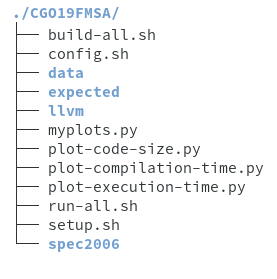
\includegraphics[scale=0.5]{figs/tree.png}
\end{figure}

In order to install all dependencies described above, run the \texttt{setup.sh}
script with \textit{sudo} privileges. That is, assuming that you are in the
CGO19FMSA directory, run the following command:
\begin{figure}[h]
\texttt{sudo sh setup.sh}
\end{figure}

Once the dependencies have been installed, run the \texttt{build-all.sh}
script to build our version of LLVM and Clang, which include our function
merging optimization as well as both the state-of-the-art optimization and LLVM's
identical function merging optimization.
Again, assuming that you are in the CGO19FMSA directory, run the following
command:
\begin{figure}[h]
\texttt{sh build-all.sh}
\end{figure}

This process might take a few hours, depending on your machine settings.
After completion, a \texttt{build} directory is created inside the CGO19FMSA
root directory.

This two scripts set up all the environment necessary to run all our experiments.

Our pre-packaged VirtualBox image (\url{http://bit.ly/cgo19fmsa-vm})
has all this environment setup and ready to run the experiments, as described
in the next section.

%%%%%%%%%%%%%%%%%%%%%%%%%%%%%%%%%%%%%%%%%%%%%%%%%%%%%%%%%%%%%%%%%%%%%
\subsection{Experiment workflow}

To run our experiments all you need to do is to execute the \texttt{run-all.sh} script
with the following command:
\begin{figure}[h]
\texttt{sh run-all.sh}
\end{figure}

This script automates the whole experiment workflow.
At the end, you should have all the expected plots, as well as the raw data as CSV files,
inside the \texttt{results} directory, which is also created inside the CGO19FMSA
root directory.

The automated process may take several hours since it involves running all following steps for all the SPEC benchmarks:

\noindent{}
\begin{itemize}
  \item Code-size measurement (Figure 10 in the paper):
\begin{itemize}
  \item Running the oracle optimization.
  \item Running the state-of-the-art and baselines optimizations.
  \item Running our optimization with all three exploration thresholds.
\end{itemize}
  \item Compilation-time measurement (Figure 11 in the paper):
\begin{itemize}
  \item Run all optimizations again, except for the oracle, multiple times in order to have a measurement with statistical significance.
\end{itemize}
  \item Execution-time measurement (Figure 13 in the paper):
\begin{itemize}
  \item Run, also multiple times, all compiled versions of the SPEC benchmarks with their reference inputs.
\end{itemize}
\end{itemize}


%%%%%%%%%%%%%%%%%%%%%%%%%%%%%%%%%%%%%%%%%%%%%%%%%%%%%%%%%%%%%%%%%%%%%
\subsection{Evaluation and expected result}

After executing the automated process described above, the \texttt{results} directory should have the following content:

\begin{figure}[h]
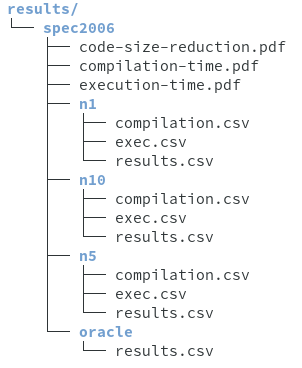
\includegraphics[scale=0.5]{figs/results.png}
\end{figure}

The main files to consider are the PDF files, which represent the plots with the
main results for the final version of our paper.
The three PDF files, as the name of the files suggest, contain the results regarding code-size reduction, compilation-time overhead,
and the performance impact of our optimization during execution-time of the benchmarks.

This artifact represents our results for the camera ready version of the paper.
We provide the \texttt{expected} results that were produced in our environment
with the up-to-date version that will be used in the camera ready version of the
paper (for example, it includes a benchmark that was missing in the original
version of our paper).
The reviewers can compare their results with the ones provided in the
\texttt{expected} directory.

%%%%%%%%%%%%%%%%%%%%%%%%%%%%%%%%%%%%%%%%%%%%%%%%%%%%%%%%%%%%%%%%%%%%%
\subsection{Notes}

To reduce the overall time required to run the full set of experiments, we have
set a small number of repetition, which may result in large error bars for some
of the benchmarks. This effect will depend on the noise of your environment.
In order to reduce the noise in the measurements, you just need to update
the \texttt{REPEAT} variable in the \textit{CGO19FMSA/run-all.sh} script,
changing it to a bigger number.

Because SPEC 2006 requires private access, in the final version, we will
change \url{http://bit.ly/cgo19fmsa-benchmark} to provide only the scripts for
running the experiments.
The source code in \url{http://bit.ly/cgo19fmsa} will remain the same.

%%%%%%%%%%%%%%%%%%%%%%%%%%%%%%%%%%%%%%%%%%%%%%%%%%%%
% When adding this appendix to your paper, 
% please remove below part
%%%%%%%%%%%%%%%%%%%%%%%%%%%%%%%%%%%%%%%%%%%%%%%%%%%%

\end{document}
